\documentclass[30pt,landscape]{foils}
\usepackage[english,german]{babel}  % language support for german/english
\usepackage[latin1]{inputenc}       % allow Latin1 characters
\usepackage{ifvtex}
\usepackage{ifpdf}
% Running vtex we most probably also create pdf...
\ifvtexpdf\pdftrue\fi
\ifpdf
\usepackage{pause}               % loads also color.sty
\usepackage{background}
\usepackage{graphicx}            % for including graphics
\usepackage{geometry}
\usepackage{hyperref}
\else
\usepackage[dvipdfm]{pause}      % loads also color.sty
\usepackage[dvipdfm]{background}
\usepackage[dvips]{graphicx}
\usepackage[dvips]{geometry}
\usepackage[dvipdfm]{hyperref}
%% The following definition is only necessary, because we use variants
%% of the same graphics file in .mps and .eps format each. The variant
%% .mps is suitable for pdflatex and dvipdfm, the variant .eps is good
%% for vlatex and pdflatex. Therefore we have to setup a preference of
%% .mps for dvipdfm.
%% matrixb?e.eps is created from matrixb?e.fig using the option -p2 of
%% fig2dev. matrixb?e.mps is created running fig2dev without such an
%% option (see the manual for PPower4).
\DeclareGraphicsExtensions{.jpg,.jpeg,.pdf,.png,.mps,.eps,.ps}
\fi
\usepackage{pp4slide}
\geometry{headsep=3ex,hscale=0.9}
\hypersetup{pdftitle={pdftexdemo},
  pdfsubject={A demonstration of LaTeX and Acrobat},
  pdfauthor={Klaus Guntermann, FG systems programming, TU Darmstadt, Germany
  <guntermann@iti.informatik.tu-darmstadt.de>},
  pdfkeywords={pdftex, acrobat},
  pdfpagemode={FullScreen},
  linkcolor={red}
  }
\begin{document}
{\Large\normalcolor\bf
  \LaTeX{} and Acrobat Reader\\
  \null\hfill for Presentations\break}

\noindent
Nowadays special programs like PowerPoint or
MagicPoint are used for presentations.\pause\\
But with some extras also \TeX/\LaTeX{} can be used to prepare
presentations, which catch the eyes of the audience.\pause\\
This document is an example how to use the FullScreen mode of Acrobat
Reader for a presentation.\pause

{\tiny
Hit Return/Enter/PageDown to go on.\hfill\pauselevel{=1}}


\foilhead{What can you expect?}
\begin{itemize}
\item First one expects to build itemized lists\pause
  \begin{itemize}
  \item which can be nested\pause
  \item and use different symbols
    \begin{itemize}
    \item even this deep\pause
    \end{itemize}
  \item back again\pause
  \end{itemize}
\item and the end of this list
\end{itemize}

\foilhead{If you like it, you can use other background}
\definecolor{bgblue}{rgb}{0.04,0.39,0.53}
\vpagecolor{bgblue}
\begin{itemize}
\item You have seen a one color background before.
\item This page has a gradient like background (expect strange results
  on displays which cannot use TrueColor).
\item Page transitions need not only be immediate...
\end{itemize}

\foilhead{More background info}
\hypersetup{pdfpagetransition=Dissolve}
\definecolor{bgmag}{rgb}{0.7,0.39,0.7}
\hpagecolor{bgmag}
...if you like such things.
\begin{itemize}
\item Background gradients can also go horizontal.\pause
\item More examples of strange color ranges are omitted here.
\end{itemize}

\foilhead[-1cm]{What is better than with PowerPoint etc.?}
\hypersetup{pdfpagetransition=R}
\vpagecolor{bgblue}
Scientific presentations are in need of formula displays in many cases.\pause\\
But the ``industry standard'' presentation tools do not help with
these very much.\pause\\
But if you prepare your presentation with \LaTeX{}, formulas are no
problem at all:
$$
  \sum_{i=0}^\infty a_i\cdot x^i
$$

\foilhead[-4.1cm]{Go through longer calculations...}
\begin{eqnarray*}
H(s) &=& \int_{-\infty}^{+\infty} h(t) e^{2\pi ist} dt\pause\\
     &=& \int_{-\infty}^{+\infty} \left\{\int_{-\infty}^{+\infty}
         f(\xi) \cdot g(t - \xi) d \xi \right\} e^{2 \pi ist} dt\pause\\
     &=& \int_{- \infty}^{+ \infty} f(\xi) \left\{ \int_{- \infty}^{+
         \infty} g(t - \xi) \cdot e^{2\pi is(t - \xi)} dt\right\}
         \cdot e^{2\pi is \xi} d \xi\pause\\
     &=& \int_{- \infty}^{+ \infty} f(\xi) G(s) e^{2\pi is \xi} d \xi\pause\\
     &=& G(s) \cdot \int_{- \infty}^{+ \infty} f(\xi)e^{2\pi is \xi} d
         \xi\pause = G(s) \cdot F(s)
\end{eqnarray*}

\foilhead[-2cm]{Links}

It is easy to \hyperlink{Ende}{skip} within a presentation, if you
want to make a side discussion or if you have to skip material.
These skips may go forward or backward.
If you click the highlighted word "`skip"' above,
you are transferred to another page of this document. Find the word
 "`Back"' on that page and click it to come back here.\pause\\
If your Acrobat Reader is configured that way, you can also link into
a web browser. Try to go to the WWW page of PPower4 by clicking
\href{http://www-sp.iti.informatik.tu-darmstadt.de/software/ppower4/}{here}.

\foilhead[-2cm]{Pictures}
\vpagecolor{bgmag}
Of course you can include pictures or diagrams and show them one by one\pause,
even mixed with text.
  \begin{center}
  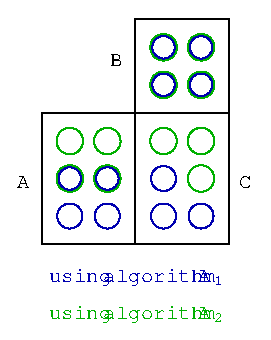
\includegraphics[scale=1.6]{matrixb1e}
  \pause\qquad\qquad
  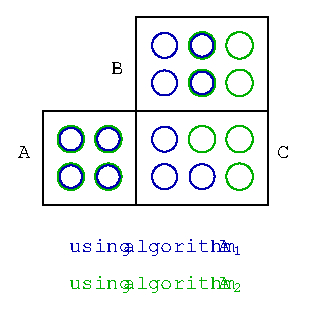
\includegraphics[scale=1.6]{matrixb2e}
  \end{center}
{\small These pictures were created with XFig, exported to MetaPost format
  and included with scaling.}

\foilhead[-2cm]{The End}
\vpagecolor{bgblue}

Thank you for going through this document.\\
You may proceed reading the
\href{http://www-sp.iti.informatik.tu-darmstadt.de/software/ppower4/report.pdf}%
{report} on PPower4, the software tool which was used to prepare this demo.
Please note that the report only describes the initial development,
not the current state.
\hypertarget{Ende}{}
\vfill

Hit \texttt{Esc} to leave FullScreen mode.\\
Select the appropriate entry in the View menu to return to this mode.\\
\hbox to \textwidth{\small\hfill \Acrobatmenu{GoBack}{Back} to
  the page displayed before.}
\end{document}
